\section{VirtualBox}\label{sec:virtualbox}
This open-source software project backed by Oracle is well-known in the virtualization industry. It is a hypervisor, a type of program defined by Red Hat as a
\begin{shadedquotation}
	[...] software that creates and runs [one or more] \gls{VM}. A hypervisor, sometimes called a \gls{VMM}, isolates the hypervisor operating system and resources from the virtual machines and enables the creation and management of those VMs.\cite{online:redhat}
\end{shadedquotation}
Indeed, VirtualBox acts as a mediator between a guest OS (the \textit{virtualized} OS) and a host OS. It is labeled as a Type-2 hypervisor, meaning that it is actually a software layer that separates both operating systems, as \autoref{fig:layerhyper} shows. VirtualBox is in charge of exposing computer utilities to the guest operating system, like CPU time, RAM allocation, driver and graphics card access, etc. Like most of its counterparts, the hypervisor also offers to the user the possibility of manually \textit{snapshotting} a virtual machine's current state in order to allow a future restore to exactly this state: the state of the drivers, running processes scheduling information, even the graphical interface. The feature outputs a sizable file as a result.

\begin{wrapfigure}{r}{0.45\textwidth}
	\centering \scriptsize
	\vspace{-12pt}
	\includesvg[width=0.37\textwidth]{svg/hypervisor}
	\caption{Abstraction layers for a type-2 hypervisor.}
	\label{fig:layerhyper}
	\vspace{-24pt}
\end{wrapfigure}
Since VirtualBox is an open-source project, anyone can have access to its source code. Consequently, it's possible to take a look at the different strategies that were taken to solve certain problems. In this case, how VirtualBox handles the saving of guest OS processes and memory is of particular interest.

Inside the code repository, the \pathmono{SnapshotImpl.cpp} file contains the relevant \Cpp classes and routines that provide the starting point for this analysis. Specifically, the \cppsym{SessionMachine::i_takeSnapshotHandler} can be recognized as the method responsible for the snapshot feature. The feature does many things, but four snapshot aspects stand out by how they approached their design to make the saving problem possible.

\subsection*{Snapshotting process}

VirtualBox needs an efficient strategy to save the general state of the virtual machine. Precisely, it is VBox's Saved State Manager's (SSM) responsibility to implement the facilities for saving and restoring a VM state in a structural manner.

During initialization of a given virtual machine (i.e right before the guest OS starts its boot sequence), the SSM registers the different virtual components that are available to the virtualized operating system. When time comes for the user to hit the \inlinegraphics{art/take-snap.png} button while the VM is running, the Saved State Manager goes through its list of registered components. The components then save their internal state themselves using the API the SSM provides, and the SSM takes care of encoding the data. As a result, what is called a "stream" in the project is produced from the agglomeration of the saved data. This is a powerful way of dealing with this problem and has many advantages :
\begin{enumerate}
	\item Encapsulation is kept since each component takes care of saving itself. This is good for software maintenance.
	\item Adding a new component to include in a save only requires it to register itself at initialization. The SSM doesn't need to be aware of the capabilities said component provides.
	\item The time to save a machine's state grows linearly with the number of components, since they are completely decoupled from each other.
\end{enumerate}

\hfill\textit{Relevant file }: \pathmono{src/VBox/VMM/VMMR3/SSM.cpp}.

\subsection*{Non-volatile Memory Snapshot}

From a hard disk point of view, the hypervisor takes a \textit{diff}-based approach. This means that from the time a snapshot is created, VirtualBox associates it with a list $L$ of changes in which all $n$  subsequent hard disk write operations $w$ are added. When the user wants to come back to a certain snapshot taken at time $t_0$, the \gls{VMM} then takes the current state of the disk ($\text{HDD}_{tn}$) and traverses $L$ in the reverse order while applying the inverse operation.
\[
\text{HDD}_{t0} = \text{HDD}_{tn} + \sum_{i=n}^{0}w_i^{-1}
\]
This effectively undos all previous operations. Using this technique means that \ul{VirtualBox snapshots are dynamic objects} that grow linearly with the subsequent usage of their affiliated VM.

\hfill\textit{Relevant file }: \pathmono{src/VBox/VMM/VMMR3/SSM.cpp}.

\subsection*{CPU State Snapshot}

As for the saving of the CPU state itself, the CPU Monitor (CM) is responsible for keeping track of all the CPU and \gls{FPU} registers while the virtual machine is running. In practice, the exact identity of all those registers depends on the architecture of the host hardware (assumed to be x86) and the host OS. For instance, a 32-bit OS would be using the "extended" (\textit{E}-prefixed) registers, like in \autoref{fig:x86-regs}. 
\begin{figure}[H]
	\centering
	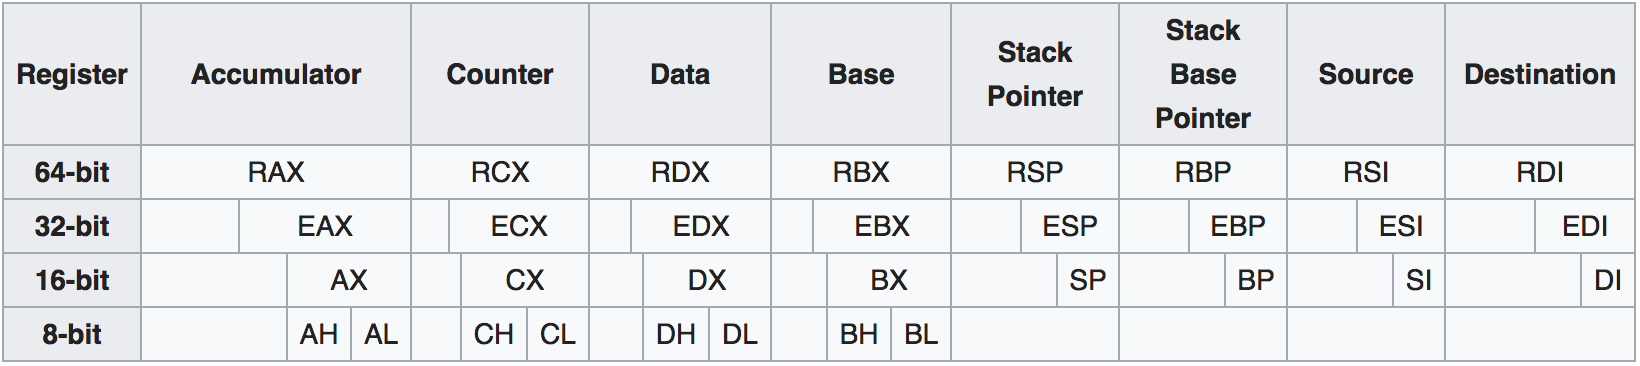
\includegraphics[width=.85\linewidth,keepaspectratio]{art/x86-regs.png}
	\caption{Usage of basic registers ordered by word size of the operating system on the x86 architecture.}
	\label{fig:x86-regs}
\end{figure}
The state (i.e value) of all the relevant CPU registers at a time $t$ is called a \textbf{context}. In VirtualBox, the CM keeps local copies of three of these contexts : a guest OS context, a special hypervisor context for the VMM and a raw context (a normal host OS context). When making a snapshot of the VM, the CPU Monitor actually saves the first two in order to subsequently put back the CPU exactly like it was at time $t$. Beside the saving aspect, holding three different contexts also allows VirtualBox to quickly switch between the guest and host "worlds" without the user noticing. This is very much necessary, because the whole point of the hypervisor is to make two different operating systems coexist at the same time.

\hfill\textit{Relevant file }: \pathmono{src/VBox/VMM/VMMR3/CM.cpp}.

\subsection*{RAM Snapshot}
Another vital aspect of the state save is the dynamic memory aspect. How can VirtualBox completely separate the guest OS from the host without the guest noticing? This is done through the Page Manager (PM), a manager also taken into account by the Saved State Manager at snapshot time. 

\begin{wrapfigure}{l}{0.45\textwidth}
	\centering \scriptsize
	\vspace{-12pt}
	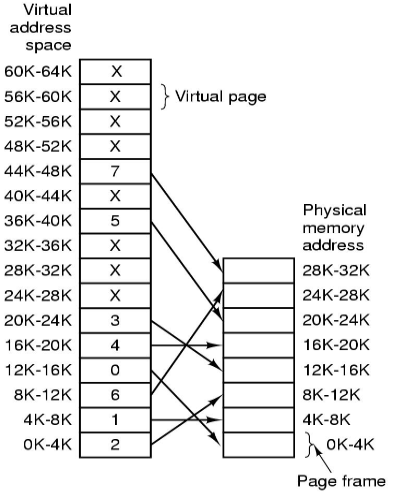
\includegraphics[width=0.40\textwidth,keepaspectratio]{art/mem-paging.png}
	\caption{Linux Mapping of Pages to Page Frames \cite{misc:mem-paging}}
	\label{fig:mem-paging}
	\vspace{-12pt}
\end{wrapfigure}
To better understand the Page Manager's job, a very similar concept can be taken as an example: the memory paging technique used by the Linux operating system. As shown in \autoref{fig:mem-paging}, the way Linux abstracts the hardware from a running program is by offering said program an entire virtual address space as a sandbox. 

This virtual space is divided into fixed-length memory blocks (usually 4kB) called virtual pages that have a one-to-one correspondence to a random block of the same size in physical memory (page frame). Linux abstracts that correspondence with the help of a \gls{MMU} implemented in hardware, which translates virtual addresses into physical ones.

In the same way that Linux controls VirtualBox's physical memory accesses, the Page Manager controls the guest OS memory accesses. It enables the management of pages of memory allocated by the guest and adds one more level of memory indirection. For example, a program running on the guest OS will be executing operations on guest memory, but VirtualBox actually redirects them to operate directly on the physical address space offered by the host OS. This can be done with the help of two powerful concepts:
\begin{enumerate}
	\item \textbf{Binary translation}. This allows a software-assisted hypervisor like VirtualBox to "trap and virtualize the execution of sensitive, non-virtualizable instructions sets"\cite{online:virtualization}, like memory operations. In other words, the guest's machine code is translated to host machine code.
	\item \textbf{\gls{SLAT}}. Also known as \textbf{nested paging}, it allows a guest operating system to directly access the host's physical memory and thus removing a lot of overhead on memory operations.
\end{enumerate} 

Because the \gls{VMM} can hook to these memory operations in the guest OS, this makes the Page Manager aware of the page frames that belong to the guest OS. As a result, when a snapshot event occurs, the PM goes through its list of guest pages that were in use at that time and saves them. At restore time, this data is copied back someplace else in physical memory, and the translation table is updated accordingly.
 
\hfill\textit{Relevant file }: \pathmono{src/VBox/VMM/VMMR3/PGM.cpp}.